\section{Problema 3: Laboratorio farmacol\'ogico}

\subsection{Introducci\'on}

\quad En un laboratorio farmacológico se trabaja con un cierto tipo de virus bastante particular. Cuando una persona contrae este virus, el mismo sufre una adaptación al individuo y muta en cierta forma según el ADN del huesped. Una persona infectada puede contagiar a otra pero sólo si comparten cierta información genética particular, la cual depende del individuo infectado. Por este motivo, podría ocurrir que una persona pueda contagiar a otra pero no al revés.

\quad El director de este laboratorio cuenta con un conjunto de investigadores a quienes debe distribuir en grupos para que trabajen con este virus. El director cuenta con la información del ADN de cada investigador y para cada investigador sabe a qué otros investigadores puede contagiar el primero. A un grupo de trabajo se lo considera de extremo riesgo si infectando a cualquiera de sus integrantes existe la posibilidad de que todos los integrantes se contagien. El objetivo del director es armar grupos de trabajo de manera que ningún grupo sea un extremo riesgo. Cada grupo trabajará independientemente de los demás, con lo cual no hay riesgo de contagio entre grupos.

\quad Considerando la situación expuesta en párrafos anteriores, se nos pidió escribir un algoritmo eficiente que detecte todos los grupos de extremo riesgo maximales en el conjunto total de investigadores. Si bien no se nos impuso ninguna cota de complejidad, se nos informó que se puede hallar un algoritmo que resuelva el problema en tiempo lineal en función del tamaño de entrada.


\subsection{Desarrollo}

\quad Dadas las características del problema a resolver, lo primero que determinamos fue cómo podíamos modelarlo. Rápidamente, caímos en la cuenta de que podemos modelar el problema mediante el uso de grafos dirigidos. De esta manera a cada investigador le corresponderá un nodo. La existencia de una arista que una dos nodos sumada a la dirección representará la posibilidad de contagio. Es decir si una arista sale de un nodo A y llega a un nodo B, se estaría indicando que el investigador A puede contagiar a B.

\quad Se definió en el enunciado que un grupo de extremo riesgo es aquél dónde infectando a un investigador cualquiera que integra dicho grupo se pueden contagiar a todos los demás. A través de un pequeño ejemplo podemos determinar qué es un grupo de extremo riesgo maximal.

\quad Supongamos un grafo con tres nodos A,B y C. De A sale una arista que se dirige a C y otra arista que se dirige a B. De C sale una arista que se dirige a A. En este ejemplo, los grupos de extremo riesgo maximales son \{A,C\} y \{B\}. Notar que los grupos \{A\} y \{C\} son también de extremo riesgo, sin embargo no son maximales.

\quad Pensando esta definición en términos del modelo que elegimos para representar el problema, es fácil observar que un grupo de extremo riesgo maximal se corresponde con una componente fuertemente conexa del grafo. Es decir, que podemos reducir el problema a determinar cuáles son las componentes fuertemente conexas del grafo dirigido que modela una instancia del problema.
 
\quad Determinar las componentes fuertemente conexas de un grafo dirigido es un problema conocido, del cual se conocen además soluciones que lo resuelvan en tiempo lineal en función de la entrada.

\quad Dos algorimos conocidos para resolver este problema son el algoritmo de Kosaraju \footnote{$http://en.wikipedia.org/wiki/Kosaraju's\_algorithm$} y el algorimo de Tarjan\footnote{$http://en.wikipedia.org/wiki/Tarjan's\_strongly\_connected\_components\_algorithm$} \footnote{$http://en.algoritmy.net/article/44220/Tarjans-algorithm$} . Es de notar que ambos surgen haciendo uso del algoritmo DFS para recorrer grafos y realizando algunas modificaciones.  Nosotromos nos decantamos por realizar una implementación del algoritmo de Tarjan. Los pormenores del algorimo se pueden hallar en la sección correspondiente del informe.

\quad Aplicando entonces nuestra implementación del algoritmo de Tarjan en la implementación de grafo que hicimos, obtendremos las componentes fuertemente conexas de dicho grafo, y por lo tanto los grupos de extremo riesgo maximales, que es lo que nos pedía el enunciado. Además, obtendremos la solución en tiempo lineal de en función de la entrada.


\subsection{Algoritmo} 

\quad Como mencionamos anteriormente hemos decidido implementar el algoritmo de Tarjan para resolver el problema. La idea del algoritmo de Tarjan es ir recorriendo a partir de un nodo el grafo. De acuerdo al orden en el que se visitan los nodos se les asigna un índice que va aumentando en uno por cada nodo recorrido. El algoritmo nunca visita de vuelta nodos que ya han sido visitados. Para determinar las componentes fuertemente conexas, la idea es encontrar el nodo $raiz$ de la componente. Un nodo $raiz$ de una componente fuertemente conexa es aquél que se visitó en primer lugar. Es menester mencionar que el concepto de nodo $raiz$ sólo tiene sentido en la apĺicación del algoritmo y no fuera de éste: en realidad una componente fuertemente conexa no tiene nodo raíz. La particularidad de un nodo $raiz$ es que al ser el primero de la componente fuertemente conexa en ser visitado su índice será menor o igual que el de todos los demás nodos de dicha componente. Luego, determinaremos que para todos los nodos de una componente fuertemente conexa vale que se puede hallar un camino simple ida y vuelta entre dicho nodo y el nodo $raiz$. 

\quad Recorremos con DFS cada subgrafo y guardamos para cada nodo un valor que hace referencia al nodo de menor índice al que se puede acceder desde él y que se llamará lowIndex (y que para cada componente fuertemente conexa se correponde con el nodo $raiz$) y se van  agregando los nodos a una pila en el orden en el que fueron recorridos. Luego, determinaremos los elementos de cada componente fuertemente conexa del grafo haciendo uso del lowIndex calculado: todos los nodos con el mismo valor de lowIndex pertenecen a la misma componente fuertemente conexa. Cuando se determinó que ya se recorrió toda la componente conexa se van desapilando los nodos de la pila y se los agrega a un vector, que contiene a todos los elementos de la componente fuertemente conexa. Este vector a su vez se agrega a una vector de vectores, que contiene las componenetes fuertemente conexas calculadas hasta ese momento.  Como esto se hace para todos los nodos, podemos estar seguros que se obtienen de esta manera todas las componentes fuertemente conexas del grafo dirigido.

\quad Queremos hacer un pequeño comentario acerca de la implementación. Dentro de la estructura que representa a un Grafo para este ejericio, definimos tres vectores de tamaño igual a la cantidad de nodos del grafo. Sabiendo de antemano que a cada nodo le corresponde un entero, definimos los vectores de la siguiente manera:

\quad El vector $indice$ guarda para cada nodo el orden en el que se lo recorrió con Tarjan. De esta manera, en la i-ésima posición del vector encontramos en índice que le corresponde al nodo $i$ de acuerdo al orden en el que se lo recorrió con el algoritmo. Si el valor de indice para un nodo es -1, entonces ese nodo no fue visitado todavía.

\quad Análogamente, el vector $indiceBajo$ guarda la información acerca de qué lowIndex le corresponde a cada nodo. En la posición $i$ del arreglo encontramos el lowIndex que le corresponde al nodo $i$ de acuerdo a la corrida del algoritmo.

\quad Finalmente, el vector $presenta$ guarda la información relativa a si un nodo se encuentra o no en la stack de la que hace uso el algoritmo de Tarjan. Así, la posición $i$ del vector contendrá un false si el nodo $i$ no se encuentra en la pila, y un true en el caso contrario.

\quad Consideramos necesario hacer esta aclaración porque haremos uso de estas estructuras en el pseudocódigo también, por cuestiones de claridad.


%%%%%%%%%%%%%%%%%%%%%%%%%%%%%%%%%%%%%%%%%%%%%%%%%%%%%%%%%%%

%PSEUDOCODIGO DEL ALGORITMO


\begin{algorithm}[H]
\caption{} 
\begin{codebox}
\Procname{$\proc{grupoDeRiesgoMaximales}()$}
\li vector$<vector<unsigned int>>$ $res$
\li unsigned int $index$
\li $stack<unsigned int> pila$
\li
\li \For $i$ desde 0 hasta CantNodos \Do
\li	\If nodo $i$ no fue visitado \Do
\li	tarjansAlgorithm($index$, $pila$, $i$, $res$)
	\End	
    \End
\End
\end{codebox}
\end{algorithm}


\begin{algorithm}[H]
\caption{} 
\begin{codebox}
\Procname{$\proc{tarjansAlgorithm} $(unsigned int index, stack$<$unsigned int$>$ $>$ pila$, \\ $unsigned int nodo$, $vector$<$vector$<$unsigned int$>>$ componentes)}
\li $indice[nodo] \gets index$
\li $bajoIndice[nodo] \gets index$
\li index++
\li pila.push(nodo)
\li $presente[nodo] \gets true$
\li 	 
\li \For cada vecino $v$ de nodo \Do
\li 	\If v no fue visitado \Do
\li		tarjanAlgorithm(index,pila, v, componentes)
\li		$bajoIndice[nodo] \gets min(bajoIndice[nodo], bajoIndice[v]$
\li	\Else 
\li		\If v está en la pila \Do
\li			$bajoIndice[nodo] \gets min(bajoIndice[nodo], indice[v])$
		\End
	\End
    \End
\li
\li \If bajoIndice[nodo]== indice[nodo] \Do
\li	vector unsigned int $comp$
\li 	\While (nodo != tope de la pila) \Do
\li		$presente[pila.top()] \gets false$
\li		agregar pila.top() al final de $comp$
\li		pila.pop()
	\End
\li	$presente[pila.top()] \gets false$
\li	agregar pila.top() al final de $comp$
\li	pila.pop()
\li 	agregar $comp$ al final de $componentes$		
 \End
\End
\end{codebox}
\end{algorithm}


%%%%%%%%%%%%%%%%%%%%%%%%%%%%%%%%%%%%%%%%%%%%%%%%%%%%%%%%%%%

\subsubsection{Análisis de Complejidad}

\quad Como se dijo anteriormente, se resuelve en tiempo lineal a la cantidad de nodos y aristas presentes en el grafo. Básicamente, es un \textit{DFS} adaptado a grafos dirigidos. Por cada vértice que se visita con DFS, se calcula índice, bajoIndice (lowLink), se lo ubica en la pila una vez, y se lo saca una sola vez. Determinar si se encuentra en la pila se obtiene con costo constante porque usamos un arreglo de booleanos. Las demás operaciones son constantes.

\quad Es muy importante tener implementado el grafo con lista de adyacencias así obtener los vecinos de un nodo se puede realizar en O(1).

\quad

\quad Robert Tarjan lo explica detalladamente en cuando presentó su solución en \textit{SIAM Journal on Computing}. \footnote{ Tarjan, R. E. (1972), "Depth-first search and linear graph algorithms", SIAM Journal on Computing 1: 146–160 Teorema 13}

\subsubsection{Correctitud}

\quad Robert Tarjan demuestra \footnote{ Tarjan, R. E. (1972), "Depth-first search and linear graph algorithms", SIAM Journal on Computing 1: 146–160 Teorema 14} la correctitud de su algoritmo en el mismo artículo mencionado anteriormente. Para ello, por inducción, demuestra que se calcula correctamente el valor de $ bajoIndice $ para cada nodo. Haciendo esto, determinar si un nodo es la la \textit{raiz} de la componen fuertemente conexa es correcto para todos los vértices. Una vez encontrada la raíz, en esa componente los vértices estan en la parte superior de la pila. Se los saca y se los guarda en una componente fuertemente conexa.

\subsection{Pruebas y Resultados}


\quad Para realizar casos de test, decidimos armar diferentes tipos tratando de la siguiente manera:

\begin{itemize}
\item \textbf{Digrafos al azar con cantidad de componentes fuertemente conexas variable y de distintos tamaños}

\quad Decidimos utilizar un criterio que dependiendo de la cantidad de nodos, se generan distintos componentes. Para cada nodo de una componente, se determina aleatoriamente con probabilidad de $ \frac{1}{2} $ si tiene arista de salida hacia cada uno del resto de los nodos de la misma componente. Generando que esa componente sea altamente probable una componente \textit{débilmente conexa} y con una probabilidad considerable de que sea \textit{fuertemente conexa}. Si bien no estimamos la probabilidad, la cantidad de componentes fuertemente conexas son alrededor de $ \frac{\vert  V \vert}{10} $.

\quad

\quad Variamos la cantidad de nodos de 3 nodos a 300 y por cada cantidad de nodos hacemos 100 repeticiones. La cantidad de aristas para un grafo de \textit{n} nodos fue obtenida en promedio ya que al ser aleatorio variaba considerablemente la cantidad. El tiempo obtenido en función de la cantidad de nodos y aristas quedó asi:

\begin{figure}[H]
	\centering
	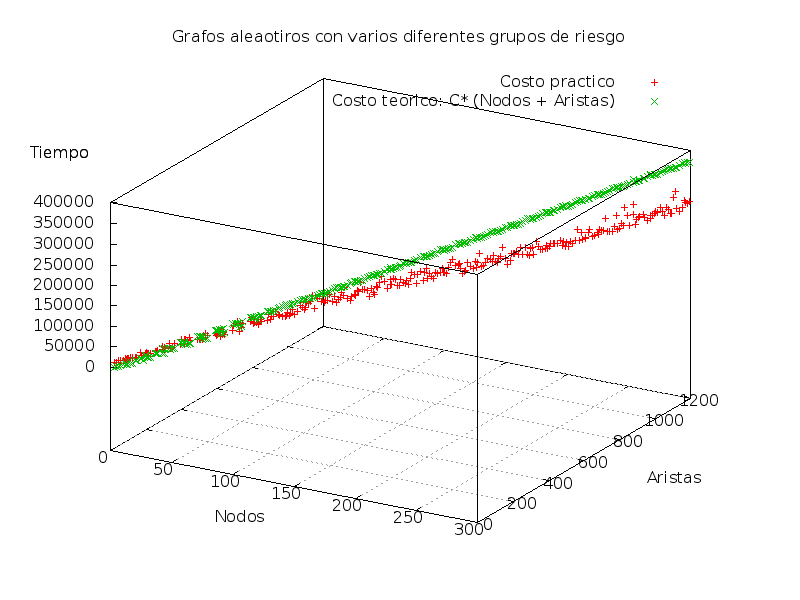
\includegraphics[scale=0.6]{ej3-grafico3.png}
\end{figure}

\quad Se observa que los costos obtenidos no superan la cota teórica obtenida en el eje z. Presentamos el siguiente gráfico a modo de aclaración de que los puntos de los costos teóricos y prácticos son los mismo en los ejes de aristas y nodos:

\begin{figure}[H]
	\centering
	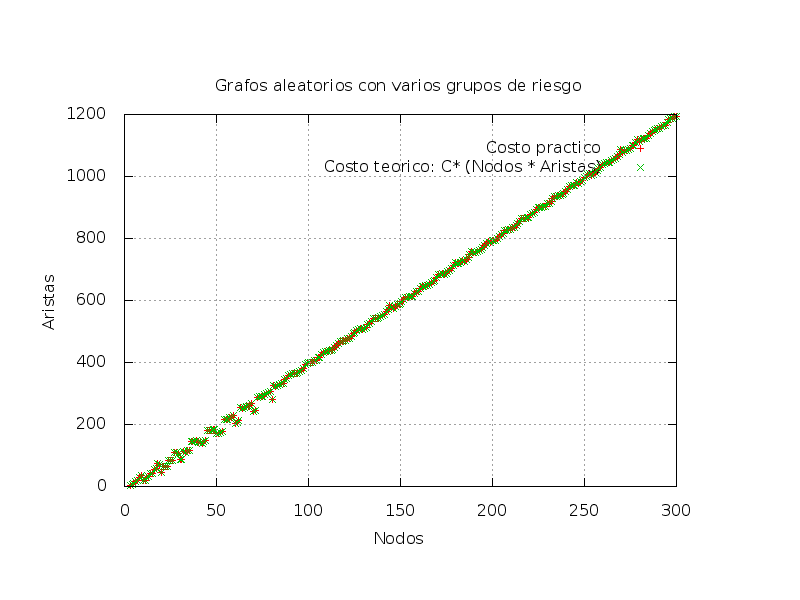
\includegraphics[scale=0.6]{ej3-grafico3-b.png}
\end{figure}

\quad Para cada valor obtenido en la curva obtenida empíricamente tiene los mismas \textit{coordenadas} en el plano de aristas y nodos, que la curva teórica podemos decir que se cumple la cota de complejidad del peor caso.

\item  \textbf{Digrafos completos, es decir, que cada nodo tiene aristas de salida a todos los otros nodos}

\quad Si bien para el ejercicio es una solución trivial, probamos como se comporta el algoritmo al tener siempre la máxima cantidad de aristas dirigidas. Por lo visto en la teórica, $ \vert E \vert = \frac{\vert V \vert * \vert V - 1 \vert}{2}$ por lo que la complejidad podría ser directamente $ C * \vert E \vert $.

\begin{figure}[H]
	\centering
	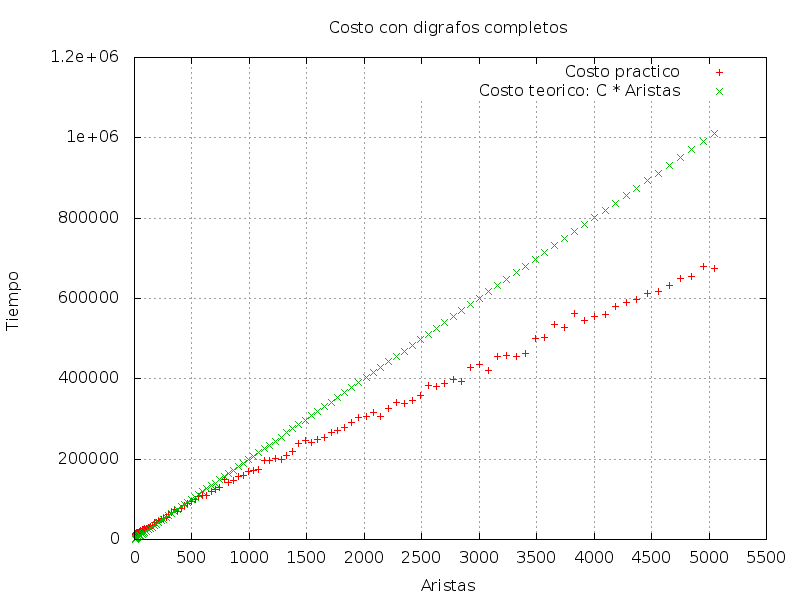
\includegraphics[scale=0.6]{ej3-grafico4.png}
\end{figure}

\quad Nuevamente, los datos obtenidos empíricamente resultan menores a la cota teórica del peor caso.

\item  \textbf{Digrafos con cantidad de nodos fija y variando la cantidad de aristas.}

\quad Como en los casos anteriores siempre se varía los nodos, decidimos hacer estos casos donde la cantidad de nodos es fija y se va variando constantemente la cantidad de aristas para cada nodo, desde 0 hasta $ \vert V - 1 \vert $. Como la cantidad de nodos es fija, la complejidad teórica en el peor caso queda: O($ C * \vert E \vert $)

\begin{itemize}

\item Con 50 nodos:

\begin{figure}[H]
	\centering
	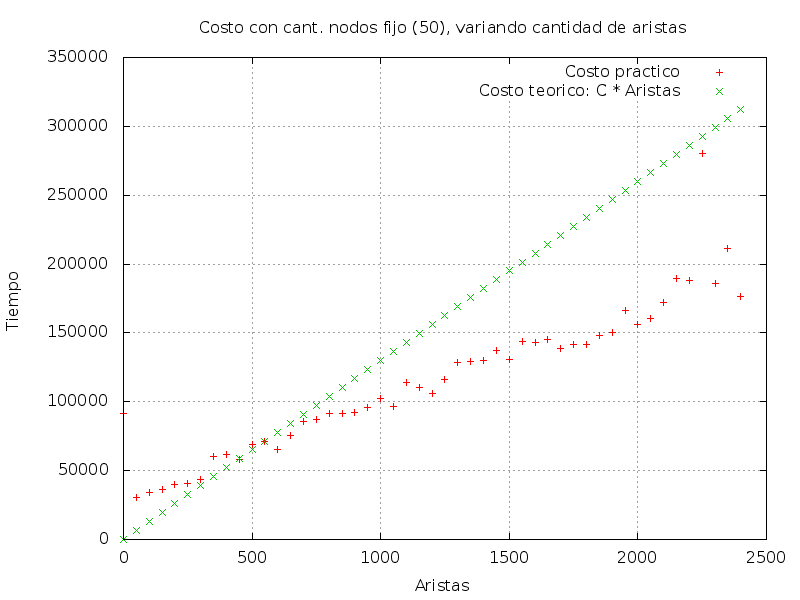
\includegraphics[scale=0.6]{ej3-grafico1.png}
\end{figure}

\quad Si bien se observa que no supera la cota lineal teórica, decidimos realizar otro test con mayor cantidad de nodos para poder obtener una mejor tendencia de los datos empíricos.

\item Con 250 nodos:

\begin{figure}[H]
	\centering
	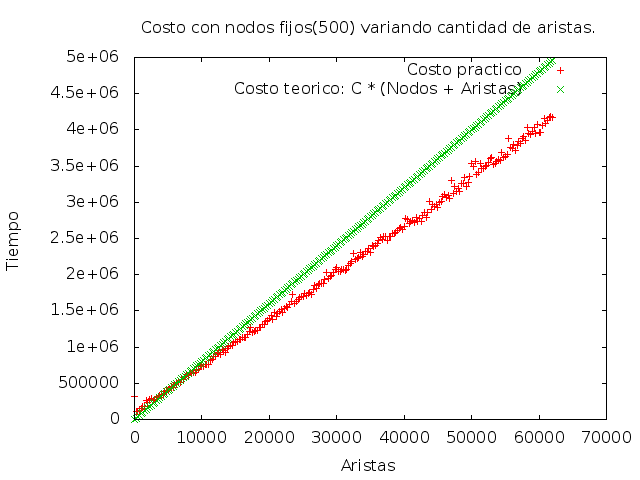
\includegraphics[scale=0.6]{ej3-grafico2.png}
\end{figure}

\quad Al ya poder observar el comportamiento del algoritmo y ver que no supera la complejidad obtenida sumado a que el test pesa 2.58 GB decidimos que esa cantidad de nodos era sufiente. Si se comprimi el test ocupa 2.24 MB.


\end{itemize}
\end{itemize}

\subsection{Conclusiones}

\quad Estudiando el problema y viendo sus posibles soluciones notamos que \textit{Depth First Search} aparece en las dos más conocidas, la de Kosaraju y la de Tarjan, entre otros. Destacamos que es crucial para poder realizar una solución lineal al problema de detectar las componentes fuertemente conexas. Llama la atención que un algoritmo simple pueda ser de gran utilidad para este y otros problemas, que hasta no muchos años no se conocia una solución lineal.
